\section{MESA} \label{appen:mesa}

Our calculations of stellar structure and evolution were performed with commit \texttt{21fd6fa} of the MESA software instrument, based upon the recent release r15140.
We patched this commit to use the version of PC which ships with MESA revision 12778 because that is more similar to the original PC EOS.
MESA uses a blend of \skye, OPAL \citep{Rogers2002}, SCVH
\citep{Saumon1995}, FreeEOS \citep{Irwin2004}, and HELM~\citet{Timmes2000}.
The blend uses \skye\ in most of the region where $T > 10^{6.2}\,\mathrm{K}$ or $\rho > 10^{4}\,\mathrm{g\,cm^{-3}}$, though the precise shape of the blend between this EOS and the others is more complicated than a simple cutoff (see Figure~\ref{fig:blend}), and was determined to minimize the the difference in energy between equations of state across the blend.

\begin{figure}
	\centering
	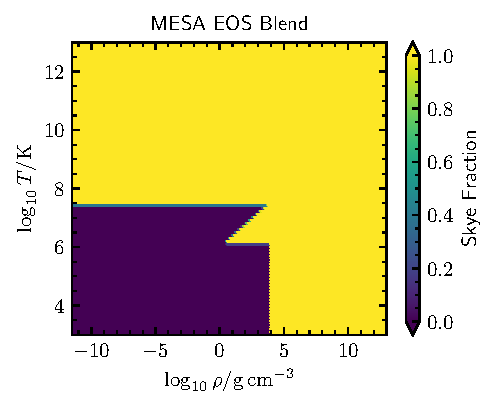
\includegraphics[width=0.45\textwidth]{skye_blend.pdf}
	\caption{The fraction of \skye\ used in the MESA EOS is shown as a function of density and temperature.}
	\label{fig:blend}
\end{figure}

Radiative opacities are primarily from OPAL \citep{Iglesias1993,
Iglesias1996}, with low-temperature data from \citet{Ferguson2005}
and the high-temperature, Compton-scattering dominated regime by
\citet{Poutanen2017}.  Electron conduction opacities are from
\citet{Cassisi2007}.

Nuclear reaction rates are a combination of rates from
NACRE \citep{Angulo1999}, JINA REACLIB \citep{Cyburt2010}, plus
additional tabulated weak reaction rates \citet{Fuller1985, Oda1994,
Langanke2000}. Screening is included via the prescription of \citet{Chugunov2007}.  Thermal
neutrino loss rates are from \citet{Itoh1996}.

\section{EOS Comparisons} \label{appen:helm}

For standalone EOS comparisons we use the version of PC which ships with MESA revision 12778, which notably smooths thermodynamic quantities across the phase transition.
This was a modification made for numerical reasons in MESA, but should not substantially affect the substance of our comparisons.
We disable Coulomb corrections in HELM and enforce full ionization across the $\rho-T$ plane.
We use the tabulated free energy for all HELM quantities, including $\partial p/\partial \rho|_T$ and $\partial^2 p/\partial\rho^2|_T$, rather than the auxiliary tables which provide these separately.
High quality numerical derivatives were determined using the $\mathrm{dfridr}$ option in the $\mathrm{eos\_plotter}$ routine in MESA.

\section{Data Availability}\label{appen:data}

The data and related scripts used in this work are available at~\citet{adam_s_jermyn_2021_4639793}.
